\chapter{Results and Analysis}
\label{ch:results}

The results follow the evidence chain established in Chapter~\ref{ch:methodology}, and are organised to answer the five research questions from \S\ref{sec:intro-rq} in turn. \S\ref{sec:benchmark-results} first checks the four clustering implementations and the label-free selection procedure on nine externally labelled datasets, before either is trusted on RetailRocket. \S\ref{sec:paired-results} then compares the fitted compact and rich partitions and their resampling stability (RQ1, RQ2). \S\ref{sec:explanation-results} compares CLASSIX provenance, ExKMC fidelity and cluster addressability (RQ3, RQ4). \S\ref{sec:sensitivity} tests whether these findings survive feature deletion, PCA, numerical perturbation, alternative session windows and a permutation control (RQ5), before \S\ref{sec:integrated-discussion} states the validity limits that bound every claim in this chapter. Throughout, each subsection reports a result, states the mechanism that plausibly produces it, gives the interpretation that mechanism supports, and marks the limitation of that interpretation — results are not left to speak for themselves.

\section{Algorithm benchmark}

Nine labelled datasets provide an algorithm check before the customer analysis. Six shape datasets and three multivariate datasets were evaluated with CLASSIX, K Means, DBSCAN and Ward. Selection used internal indices and deployment guards. Reference labels entered only the subsequent ARI and NMI calculation.

No method dominates the benchmark. K Means has the highest mean ARI across the nine selected results at 0.597, followed by Ward at 0.575, DBSCAN at 0.509 and CLASSIX at 0.508. CLASSIX and Ward share a mean rank of 2.44, while K Means has 2.39 and DBSCAN has 2.72. These averages conceal marked dependence on shape. CLASSIX recovers the Jain reference exactly but reaches only 0.264 ARI on R15. DBSCAN recovers Spiral exactly and performs best on Aggregation and Compound, yet its selected Wine candidate has no valid internal score. K Means is strongest on Seeds and Wine, while Ward is strongest on R15.

\begin{table}[htbp]
\centering
\caption{Highest external ARI after label free selection on each benchmark dataset}
\label{tab:benchmark_winners}
\begin{tabular}{lcc}
\toprule
Dataset & Method & ARI \\
\midrule
Aggregation & DBSCAN & 0.910 \\
Compound & DBSCAN & 0.826 \\
Iris & CLASSIX and K Means & 0.568 \\
Jain & CLASSIX & 1.000 \\
Pathbased & CLASSIX & 0.497 \\
R15 & Ward & 0.804 \\
Seeds & K Means & 0.481 \\
Spiral & DBSCAN & 1.000 \\
Wine & K Means & 0.897 \\
\bottomrule
\end{tabular}
\end{table}

Observed runtime depends on implementation and dataset size. Median selected runtime is 0.011 seconds for CLASSIX, 0.064 seconds for K Means, 0.003 seconds for DBSCAN and 0.004 seconds for Ward on the recorded machine. These values do not establish a universal speed ordering. The benchmark instead verifies that the implementations, label-free selector and external evaluation recover varied successes and failures before the same metric code is applied to RetailRocket. The customer conclusion rests on paired evidence rather than algorithm superiority.

\section{Representation and customer cluster structure}
\label{sec:paired-results}

This section answers RQ1 and RQ2 (\S\ref{sec:intro-rq}): how much do independently selected K Means and CLASSIX partitions agree across the two representations, and does that agreement coexist with high within-representation stability?

\textbf{Result.} Changing the represented information alters the selected customer structure for both clustering methods. Table~\ref{tab:customer_results} reports the independently selected deployment-acceptable configurations. K Means selects four clusters in each representation, but the agreement between the two four-cluster partitions is only 0.014 ARI. CLASSIX selects two compact clusters and three rich nonnoise clusters with 218 additional noise assignments (customers CLASSIX did not place in any final cluster, as defined in \S\ref{sec:classix-math}). Their cross-representation agreement is 0.068 ARI. Recall from \S\ref{sec:intro-content} that these ARI values compare the compact-space and rich-space partitions of the \emph{same} customers to each other, not to any external ground truth; both values are close to the score two unrelated random partitions of the same customers would obtain by chance, even though the customer identifiers and algorithm families are unchanged.

\begin{table}[htbp]
\centering
\caption{Deployment acceptable clustering results on the shared purchaser cohort. Noise records customers CLASSIX did not assign to any final cluster because no aggregation group containing them met the minimum-size or merging conditions to become one (\S\ref{sec:classix-math}); K Means never produces noise. Stability is mean fixed-parameter overlap-resampling ARI across ten resampled pairs (\S\ref{sec:resampling-explanation}).}
\label{tab:customer_results}
\begin{tabular}{llrrrrr}
\toprule
Representation & Method & Clusters & Noise & Largest share & Silhouette & Stability \\
\midrule
Compact & CLASSIX & 2 & 0 & 0.909 & 0.595 & 0.985 \\
Rich & CLASSIX & 3 & 218 & 0.898 & 0.291 & 0.965 \\
Compact & K Means & 4 & 0 & 0.664 & 0.560 & 0.988 \\
Rich & K Means & 4 & 0 & 0.579 & 0.351 & 0.995 \\
\bottomrule
\end{tabular}
\end{table}

\textbf{Mechanism.} \S\ref{sec:kmeans-math} and \S\ref{sec:classix-math} give the mechanical reason for this disagreement: both methods compute Euclidean distances (K Means directly; CLASSIX via its principal-direction projection) over \emph{all} standardised dimensions at once, so adding nine standardised behavioural dimensions changes every pairwise distance between customers, even though each customer's three original purchase coordinates are numerically unchanged. A different set of distances can move K Means's optimal centroids to different locations, and can change the covariance structure that determines CLASSIX's sorting direction — both of which can change the resulting partition without any change to the underlying customers.

The internal indices do not move in a single direction. Compact CLASSIX has silhouette 0.595, Davies Bouldin 1.057 and Calinski Harabasz 4285.5. The rich result has silhouette 0.291, Davies Bouldin 0.859 and Calinski Harabasz 1516.9. These CLASSIX values are calculated on each partition's nonnoise observations. Davies Bouldin favours the rich result, while silhouette and Calinski Harabasz favour the compact result. Compact K Means has silhouette 0.560 and Calinski Harabasz 10459.1, compared with 0.351 and 3923.4 in the rich space. Davies Bouldin rises from 0.775 to 1.040. Richer behaviour produces a different geometry whose apparent quality depends on the criterion.

\begin{figure}[htbp]
\centering
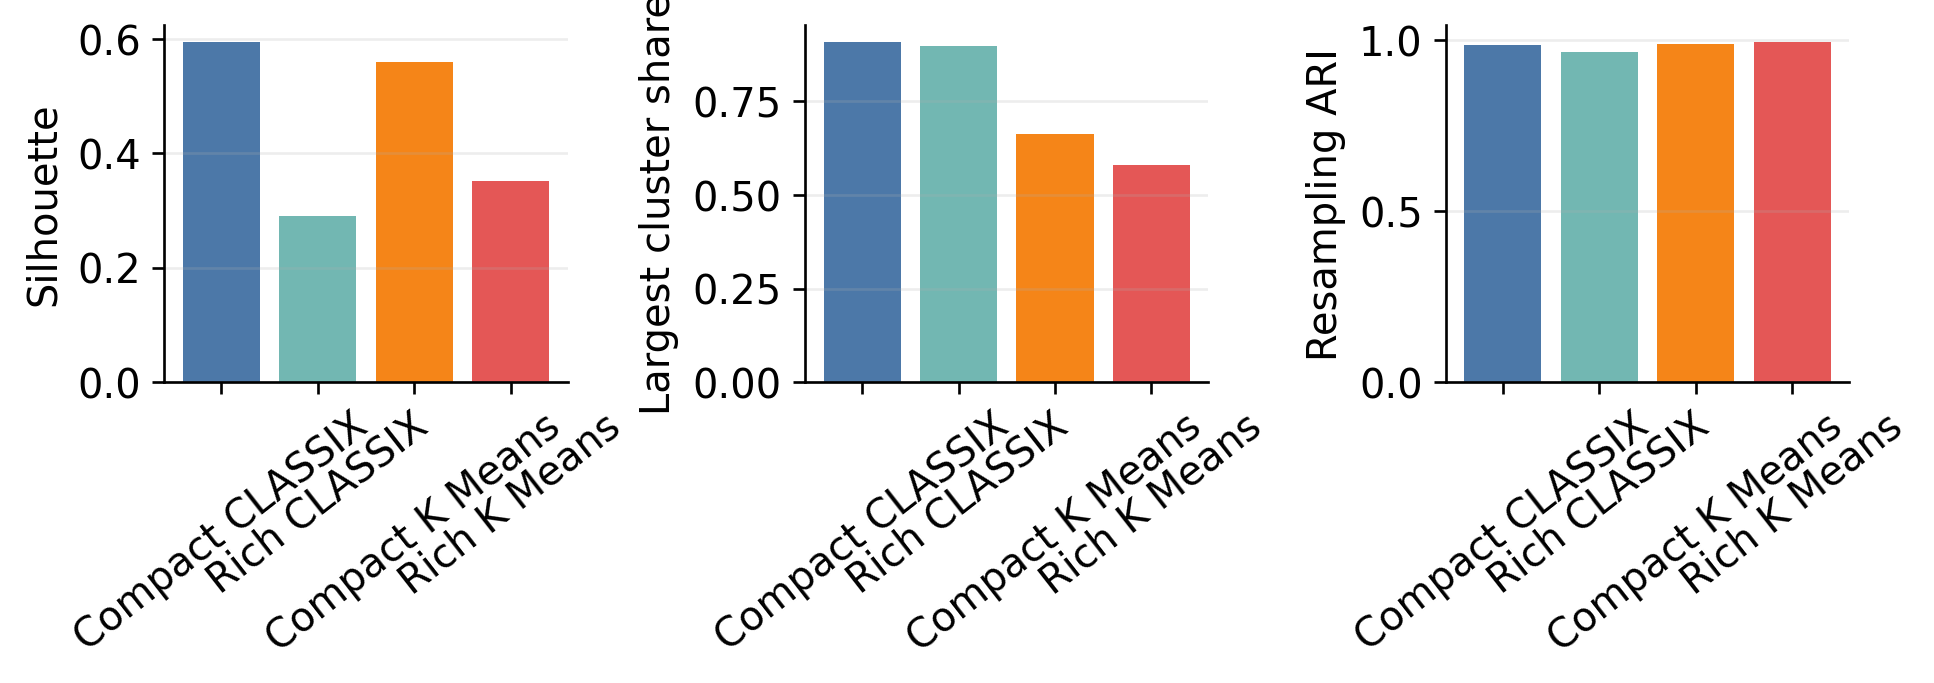
\includegraphics[width=0.80\textwidth]{figures/customer_structure.png}
\caption{Internal structure and resampling stability for the selected customer partitions}
\label{fig:customer_structure}
\end{figure}

The deployment rule materially changes the result that would be chosen by silhouette alone. Compact CLASSIX reaches silhouette 0.899 by placing 11,698 of 11,719 customers in one cluster. Rich CLASSIX reaches 0.792 with 11,716 customers in one cluster and the remaining three customers split across two tiny clusters. Compact K Means reaches 0.850 with 11,593 customers in one of two clusters. All three partitions fail the maximum share rule. The deployment selections sacrifice these high silhouette values to avoid reporting a nearly undivided customer base as a useful segmentation. Rich K Means is the only case where the unconstrained and deployment selections coincide.

Low agreement is not caused only by choosing different numbers of clusters. At every fixed K from 2 to 12, the K Means ARI between compact and rich representations remains between 0.012 and 0.113. At the common selected value of four it is 0.014, with NMI 0.089 and variation of information 1.691 nats. Under matched labels, 54.61 per cent of customers move to a different K Means cluster. Among 41 CLASSIX settings that are deployment acceptable in both spaces, matched-parameter ARI ranges from $-0.051$ to $0.392$ with a median of $-0.023$. The independently selected CLASSIX partitions have NMI 0.054 and variation of information 0.693 nats, with 18.66 per cent assigned to a different matched cluster or noise state. The lower CLASSIX migration share partly reflects the dominance of one large cluster in both representations and should not be read as stronger substantive agreement.

Cluster sizes make the changes more concrete. Compact K Means contains 7,784, 2,494, 1,344 and 97 customers. Rich K Means contains 6,790, 3,607, 1,156 and 166. Its 166 customer cluster has a median of 338.5 total events, 28 sessions and 12 top categories, whereas the full cohort medians are 6 events, 2 sessions and 1 top category. Another rich cluster of 1,156 customers has no known category at its median and a purchase recency median of 127.4 days. These are descriptive contrasts in observed features, not customer identities or causal segments.

CLASSIX yields a sharper imbalance. The compact deployment result contains 10,656 and 1,063 customers. The rich result contains 10,331, 1,137 and 33 nonnoise customers plus 218 noise assignments. The 33-customer cluster is highly active, with medians of 869 total events, 36 sessions and 14 top categories. Its small size fails the documented addressability size rule. The 1,137-customer cluster has zero category coverage and fails the coverage rule. The dominant 10,331-customer cluster has no two sufficiently distinctive median effects. Richer features expose unusual behavioural combinations, but the selected CLASSIX partition does not turn them into a balanced set of directly addressable clusters.

Fixed-parameter overlap-resampling indicates that these structural differences are reproducible under the stated sampling scheme. Mean overlap ARI is 0.985 for compact CLASSIX and 0.965 for rich CLASSIX. The corresponding K Means values are 0.988 and 0.995. The lowest of ten pairwise values is 0.881 for compact CLASSIX and 0.941 for rich CLASSIX.

\textbf{Interpretation.} This is the answer to RQ2: high within-representation stability and low cross-representation agreement are not contradictory, because they answer different questions. Stability (\S\ref{sec:resampling-explanation}) asks whether the \emph{same fixed recipe} reproduces a similar partition when refit on a slightly different 80 per cent of customers; cross-representation ARI asks whether \emph{two different recipes} (compact and rich) agree on the \emph{same} customers. A configuration can be highly self-consistent — reliably rediscovering its own partition under resampling — while still describing a genuinely different grouping from the other representation's equally self-consistent partition. This is direct evidence that representation is a modelling choice with its own reproducible consequences, not a preprocessing detail whose effect washes out once a method is "properly" fitted.

\textbf{Limitation.} Stable refitting does not imply that a partition is uniquely correct, that model \emph{selection} (choosing this configuration from the full grid in the first place) would recur under resampling, or that either partition would remain stable outside this cohort or over calendar time. It shows only that each selected representation and parameter combination tends to reproduce its own assignment pattern when one fifth of the cohort is omitted.

\section{Explanation complexity, fidelity and addressability}
\label{sec:explanation-results}

This section answers RQ3 and RQ4 (\S\ref{sec:intro-rq}): how does representation change CLASSIX's intrinsic provenance and ExKMC's post hoc fidelity, and which resulting clusters are operationally addressable? The explanation results separate provenance from approximation throughout: CLASSIX exposes how its own observations are aggregated and merged (\S\ref{sec:classix-math}); ExKMC approximates a separately fitted K Means predictor with axis-aligned rules (\S\ref{sec:resampling-explanation}). Their numbers answer different questions about different objects (\S\ref{sec:lit-gap}) and are never combined into one explanation score.

\textbf{Result (CLASSIX provenance).} The selected compact CLASSIX fit produces 131 aggregation groups that merge into two final clusters. The rich fit produces 559 groups and four final states consisting of three clusters and noise. Every exported customer trace contains the visitor identifier, aggregation group, representative row and final cluster. Both exports reproduce the selected full data labels exactly with ARI 1, confirming the trace is a faithful record of the fitted partition rather than a separate approximation of it.

\textbf{Mechanism and interpretation.} Rich CLASSIX needs more than four times as many aggregation groups even though its final nonnoise cluster count rises only from two to three. This follows directly from the staged process in \S\ref{sec:classix-math}: with nine more standardised dimensions contributing to every pairwise distance, fewer customers fall within a fixed aggregation radius $r$ of any one starting point, so more, smaller groups are needed before the merge step consolidates them into clusters. Group count is therefore a measure of local geometric granularity and computational provenance, not of how difficult the resulting clusters are for a person to read or act on — a large group count does not imply a confusing explanation, only a more finely subdivided intermediate trace.

\textbf{Result (ExKMC fidelity).} The main ExKMC comparison fixes $K$ at four for both representations because both primary K Means selections contain four clusters. At the four-leaf budget, both trees use four effective rules with depth 3 and 2.25 conditions per rule. Compact mean training fidelity is 0.9466 and mean held-out fidelity is 0.9448. Rich fidelity is higher at 0.9639 and 0.9650. Across the five splits, compact held-out fidelity ranges from 0.9416 to 0.9480 and rich fidelity ranges from 0.9599 to 0.9697. This is descriptive split variability rather than inferential uncertainty. The close training and test values give no sign of a training-only gain that disappears on held-out customers.

Compact rules use purchase occasion count and purchase recency across all five splits. Rich rules use purchase occasion count, activity span and the number of distinct top categories. Thresholds are exported in original units after reversing the training scaler and logarithmic transform. Named thresholds support direct database style conditions, but they inherit the meaning and missingness limits of the constructed variables.

\begin{figure}[htbp]
\centering
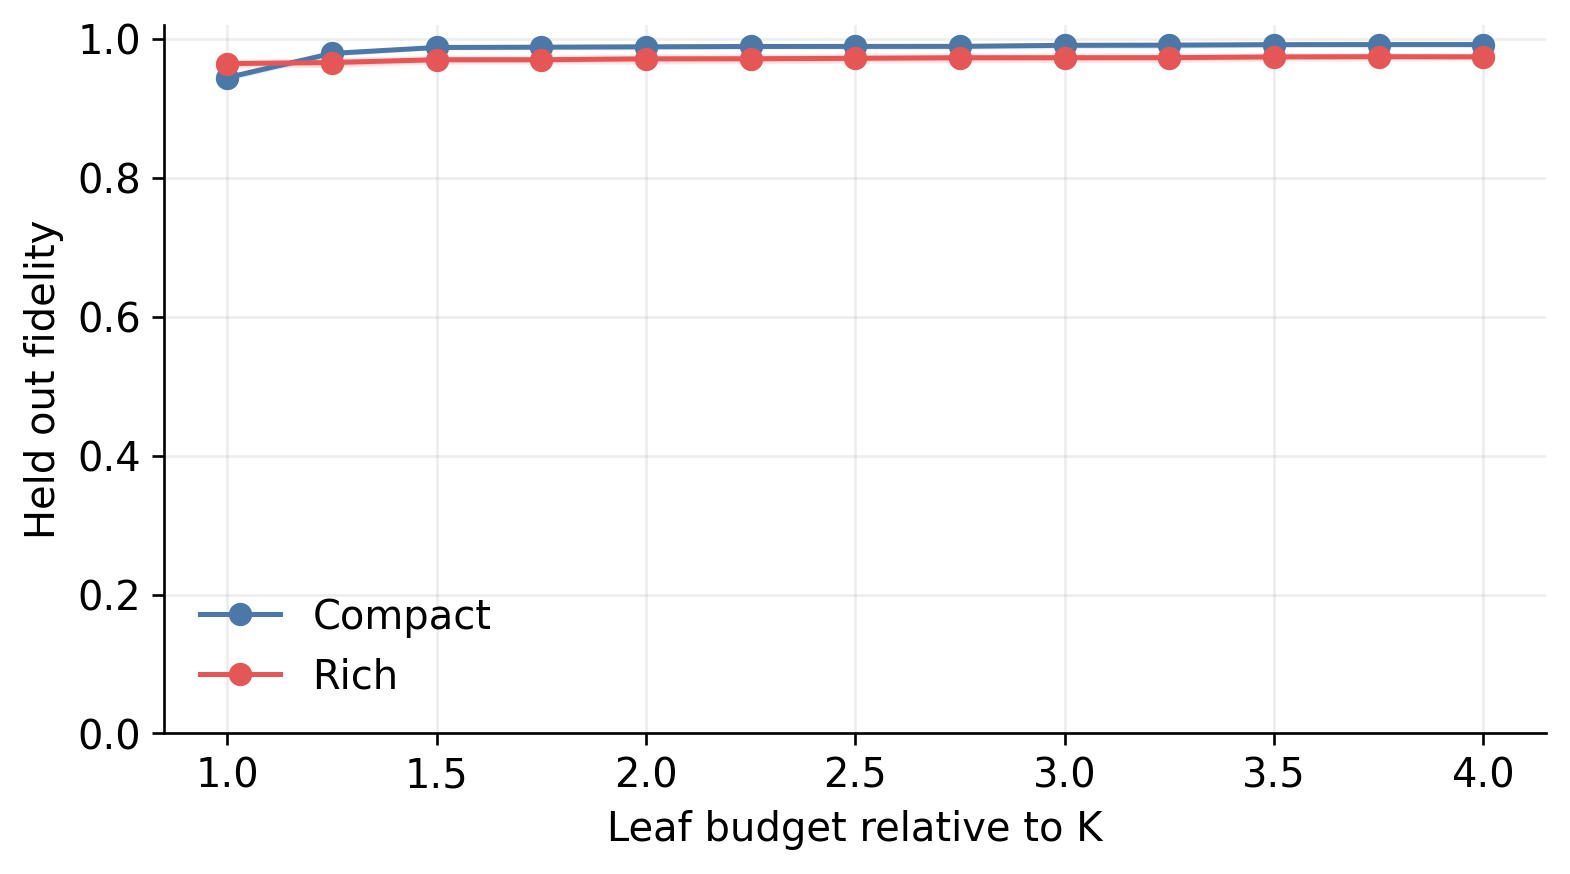
\includegraphics[width=0.75\textwidth]{figures/exkmc_tradeoff.png}
\caption{Held out ExKMC fidelity across the fixed leaf budget}
\label{fig:exkmc_tradeoff}
\end{figure}

Additional leaves change the two fidelity frontiers differently. At sixteen leaves, compact mean held out fidelity reaches 0.9924 with mean depth 6.6 and 4.84 conditions per rule. Rich fidelity begins higher at four leaves but reaches 0.9747 with mean depth 6.4 and 4.74 conditions at sixteen leaves. Compact fidelity begins lower and gains more from expansion. A supplementary training only selection chooses two compact clusters and four rich clusters in every split. Its compact fidelity is 0.9985 with two rules, but that result is not used for the main complexity comparison because $K$ differs.

\textbf{Interpretation.} The crossover between the two fidelity curves — rich ahead at a four-leaf budget, compact ahead by sixteen leaves — shows that representation changes not only \emph{whether} a small tree can approximate K Means well, but the entire \emph{shape} of the complexity/fidelity tradeoff, not merely a single headline number.

\textbf{Limitation.} A higher ExKMC fidelity is evidence that the tree agrees more often with its own K Means reference; per \S\ref{sec:lit-complexity}, it is not evidence that the underlying K Means partition is itself more correct, more useful, or more stable, since fidelity is defined entirely relative to that partition.

\subsection{Addressability: a stricter, distinct criterion}
\label{sec:addressability-hierarchy}

The preceding results show that a cluster can exist, be internally well separated (high silhouette or Calinski--Harabasz), and be highly reproducible under resampling (\S\ref{sec:paired-results}), while still failing to be usable as a targeted business segment. This dissertation therefore treats \emph{addressability} (\S\ref{sec:candidates}) as the last, and strictest, link in a chain of increasingly demanding properties: a partition can \textbf{exist} (any candidate that runs to completion); be \textbf{internally separated} (pass the silhouette/Davies--Bouldin/Calinski--Harabasz validity checks); be \textbf{stable} (survive fixed-parameter overlap-resampling, \S\ref{sec:paired-results}); be \textbf{rule-expressible} (approximated by a short ExKMC tree, or traced by CLASSIX provenance, above); be \textbf{addressable} (pass the size, coverage and distinctiveness audit); and, beyond anything measured in this dissertation, have \textbf{realised business value} (demonstrated to change an intervention outcome). Each property is necessary for the next but not sufficient for it, and this dissertation's evidence stops at addressability.

\textbf{Result.} The addressability audit is stricter than rule export, and most selected clusters fail it despite having already passed the earlier, weaker checks. Neither compact CLASSIX cluster passes because neither differs from the cohort median on at least two named features by the required half interquartile range. In the rich result, the 33-customer cluster is too small, the 1,137-customer cluster has zero category coverage, and the 10,331-customer cluster lacks two sufficiently distinctive median conditions. None of the five nonnoise CLASSIX clusters is classified as addressable. No compact K Means cluster passes. One of four rich K Means clusters passes all gates, while the others fail because they have too many distinguishing conditions or insufficient category coverage.

\textbf{Interpretation.} The compact CLASSIX partition (Table~\ref{tab:customer_results}) has the highest silhouette of any selected configuration in this dissertation, yet zero of its clusters are addressable; the rich K Means partition has the lowest compact-comparison silhouette among the four selected configurations, yet it is the only one to produce an addressable cluster. Internal validity and addressability are evidently not the same property and do not even rank configurations in the same order — a result that could not be seen without evaluating both explicitly.

\textbf{Limitation.} Business interpretation remains narrow at every stage of this hierarchy. Rich features expose a high-activity minority and a group with missing category histories, described here only as observed contrasts in recorded behaviour. ExKMC shows that K Means assignments \emph{can} be represented with a small number of named thresholds at high held-out fidelity; it does not show that a person will find those thresholds meaningful. The one passing rich cluster meets a technical audit rather than an outcome test. The observed value in this dissertation is limited to queryability and auditable coverage — the fifth link in the chain above. Revenue effect, campaign response and human comprehension, the sixth link, remain entirely unmeasured and are not claimed.

\section{Sensitivity and robustness}

Fixed-parameter checks test local dependence; reselection repeats the candidate search and deployment rule. Permutation examines additional dimensions without aligned customer information.

\subsection{Named features and reduced geometry}

Fixed parameter deletion identifies category behaviour as the strongest local influence on the rich partitions. Removing distinct top categories reduces agreement with the full rich result to ARI 0.189 for CLASSIX and 0.516 for K Means. Removing top category share gives ARI 0.238 and 0.517. Every other CLASSIX deletion remains between 0.927 and 0.967. The corresponding K Means values remain between 0.855 and 0.991. Activity span and mean interevent time have the next largest effect on K Means, with ARI 0.874 and 0.855. Influence is unevenly distributed across the named variables, but category information alone does not generate a preferable segmentation.

The PCA diagnostic preserves 91.32 per cent of standardised rich variance in six components. It is a fixed-parameter local diagnostic rather than PCA-space model selection. K Means in this reduced space agrees with the named rich partition at ARI 0.995 and has silhouette 0.390 compared with 0.351. CLASSIX retains three clusters, lowers noise from 218 to 71 customers and agrees with the named result at ARI 0.920. Its silhouette is 0.304 compared with 0.291. Mean resampling ARI is 0.995 for reduced K Means and 0.987 for reduced CLASSIX. Much of the rich partition therefore survives dimension reduction, without proving that redundancy is irrelevant or six components optimal. Rotated components lose the direct meaning needed for named-feature explanations.

\begin{figure}[htbp]
\centering
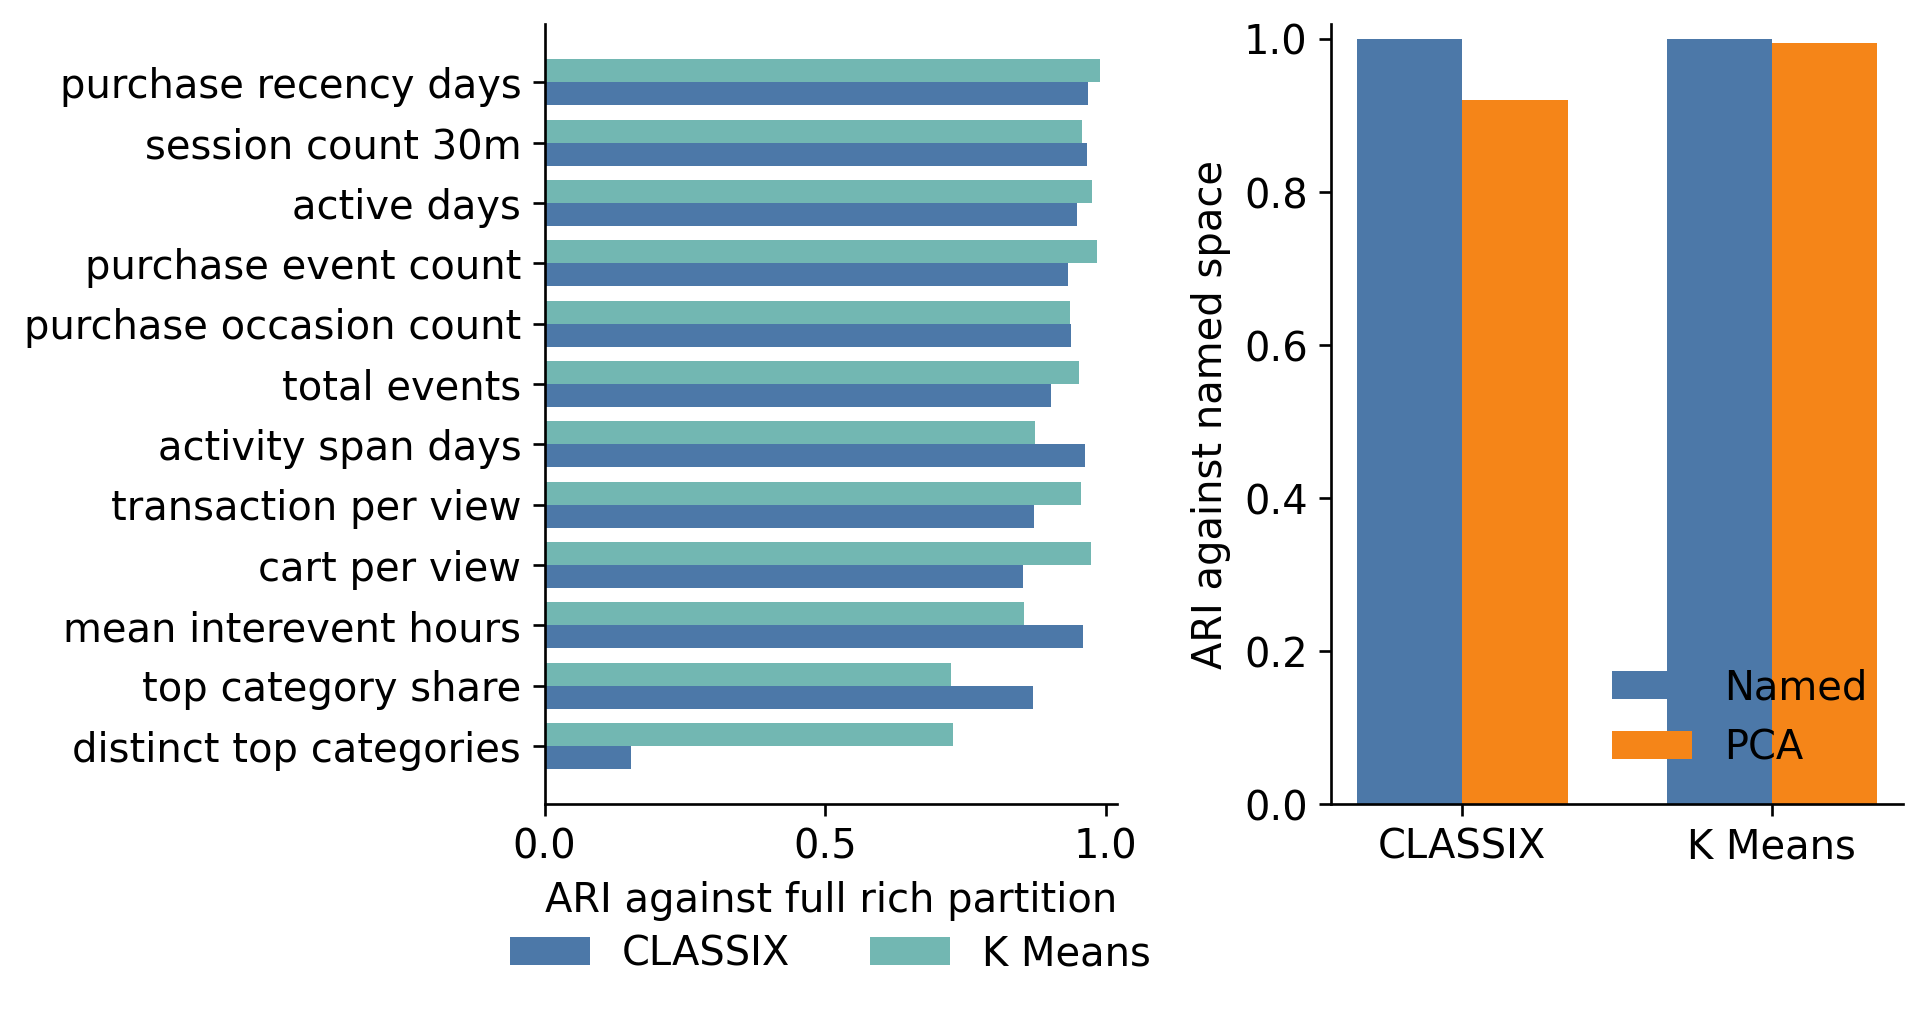
\includegraphics[width=0.80\textwidth]{figures/sensitivity_summary.png}
\caption{Reselected feature deletion and PCA diagnostics}
\label{fig:sensitivity_summary}
\end{figure}

Complete reselection confirms that category information creates the largest structural turn. All twenty two scenarios produce a deployment acceptable candidate. Removing distinct top categories changes CLASSIX to eleven clusters with ARI 0.153 against the full rich partition. K Means changes to two clusters with ARI 0.728. Removing the whole category block produces seven CLASSIX clusters with ARI 0.126 and two K Means clusters with ARI 0.729. The progressive endpoints reproduce the compact and rich primary partitions exactly. These 4,334 candidate fits show that the category effect persists when parameters and cluster counts are allowed to change.

CLASSIX sensitivity is distributed across the grid rather than concentrated at one radius. Deployment acceptable candidates occur at twenty three of thirty one compact radii from 0.35 to 1.45 and twenty rich radii from 0.30 to 1.25. Minimum size 1 produces no acceptable candidate in either representation. Minimum sizes 5 and 10 produce 23 and 32 acceptable compact candidates, compared with 19 and 27 rich candidates.

\subsection{Perturbation and temporal assumptions}
\label{sec:perturbation_results}

Small Gaussian perturbations leave the selected CLASSIX partitions almost unchanged. Compact agreement remains ARI 1 through a noise standard deviation of 0.001. At 0.01 the mean ARI is 0.999 and the minimum is 0.996. Rich agreement is also exact through 0.0001. It falls to a mean of 0.995 at 0.001 and 0.985 at 0.01, with minima of 0.985 and 0.962. Rich assignments are more sensitive at the tested scales, without wholesale reassignment. These trials cannot certify all nearby inputs. In particular, the rich fit uses density merging, outside the distance-only certificate of Section~\ref{sec:local_certificate}.

Reconstructing sessions from raw events gives a similar qualified result. The selected thirty minute window reproduces both partitions exactly. A fifteen minute window gives ARI 0.976 for K Means and 0.971 for CLASSIX. A sixty minute window gives ARI 0.985 and 0.959. The four cluster K Means result and the three cluster CLASSIX result persist at both alternative windows, although the CLASSIX noise count changes from 218 to 220 and 239. The conclusions do not arise solely from choosing exactly thirty minutes, while the detailed assignments still depend on the session convention.

\subsection{Dimensionality control}

The permutation control sets a stricter boundary on causal interpretation. The compact columns remain unchanged while the nine additional dimensions are independently permuted across customers. These columns preserve their marginal distributions but destroy their joint relationship with the compact representation and with each other. With the compact K Means setting held fixed, adding all nine permuted columns lowers agreement with the compact partition to ARI 0.017 and silhouette to 0.127. With the compact CLASSIX setting held fixed, adding even one permuted dimension produces a single cluster and ARI 0.

The single deterministic permutation control is an existence demonstration rather than a variance decomposition. Standardisation gives each added variable comparable weight, so random added dimensions can alter distances, principal directions and radius neighbourhoods in at least one realised order. The control does not estimate how much of the observed compact-to-rich difference is caused by dimensionality. Named feature deletion and PCA separately show that category and temporal information contribute reproducible structure in the observed rich representation.

\section{Integrated discussion and validity limits}

\paragraph{Strongly supported findings}
For both algorithms, representation materially changes assignments on the same purchasers, including under matched parameters. High within-space repeatability does not contradict between-space disagreement. Explanation also changes: rich CLASSIX has more aggregation groups, while ExKMC's relative fidelity reverses as its budget increases. The single passing rich K Means cluster demonstrates why geometry, repeatability, rule approximation and operational addressability require separate evidence.

\paragraph{Conditionally supported findings}
Deletion and reselection identify category dependence; PCA preserves much fitted structure, and tested numerical changes and session windows retain substantial agreement. These findings concern specific diagnostics, not all preprocessing choices. The permutation demonstrates a possible dimensionality effect without quantifying its causal share. Deployment cutoffs are operational choices; resampling holds selected parameters fixed; benchmark rankings need not transfer to purchasers. The local certificate requires unmeasured margins and excludes density merging.

\paragraph{Unresolved questions and evidence limits}
One anonymous purchaser log cannot establish general customer types. Category joins cover 76.16 per cent of events; 1,168 purchasers have no known category, and zero ratios can reflect absent recorded views. No demographic, price, revenue or response data justify labels such as valuable or loyal.

Neither intrinsic provenance nor agreement with a K Means predictor measures human comprehension. Addressability checks size, coverage and named-feature distinctiveness, not commercial outcomes. Prospective interventions and user evaluation would be needed to establish those benefits. The contribution is the joint examination of separate clustering and explanation properties under representation change, not universal superiority of richer features.

